\chapter{Existing research and references}

\section{About constructed languages in general}

"Constructed languages have long fascinated the general public, and they are now attracting
increasing attention from linguists as well. The intertwined histories of these languages and
linguistics deserve to be more widely recognized, and as discussed above, these languages have
many properties that could make them intriguing topics for linguistic research."
\footcite{goodall2023constructed} \newline

This quote, by \citeauthor{goodall2023constructed} in \citetitle{goodall2023constructed}'s conclusion,
makes a point that resonated with me quite a lot. What used to be a niche subject, only interesting
to a few scholars (or a lot of "geeks", in the case of artistic languages created for fiction like
"The Lord of the Rings"), is now a topic of interest for researchers in the field of linguistics.
Of course, as a speaker of Esperanto since adolescence, some might say that \citeauthor{goodall2023constructed}
might be slightly biased in saying this. However, I believe that on the contrary it puts the author
at a spot where they are primarily concerned with the subject, and gives them a perspective from "both
sides". \newline

In \citetitle{oostendorp2001constructed} \footcite{oostendorp2001constructed},
\citeauthor{oostendorp2001constructed} agrees with this notion and goes even further: he suggests that
most researchers dismiss constructed languages other than Esperanto on the basis that it is the only
constructed language which has risen to the level of having native speakers, or worse dismiss the field
of interlinguistics (the study of constructed/planned languages) altogether. To dispel this attitude,
\citeauthor{oostendorp2001constructed} proposes a classification of constructed languages into two categories:
"possible languages" and "impossible languages", where the former have "the potential to grow into an actual language".

This binary view of constructed languages is a simplification of the classification created by \citeauthor{blanke1989planned}
in an article which was already mentioned in Chapter \ref{chap:context}. In \citetitle{blanke1989planned}
\footcite{blanke1989planned}, \citeauthor{blanke1989planned} suggests a rather complete framework of classification,
which allows to create a real "taxonomy" of constructed languages.\newline

\citeauthor{blanke1989planned} suggests that a constructed language has to go through nineteen steps to achieve
the status of "functioning" language, and that before that they can be classified as "projects" (if they reach
step 4) or "semilanguages" (if they reach step 9).\newline

The steps \citeauthor{blanke1989planned} lists are as follow:

\begin{itemize}
    \item 1. Publication of the language's structure;
    \item 2. Production of texts in that language, sometimes published in articles;
    \item 3. International correspondance, to kickstart the socialization process;
    \item 4. Organization of the language's adepts;
    \item 5. Creation of literature;
    \item 6. Appearance of small journals;
    \item 7. Application to specialized texts;
    \item 8. Structured education of the language;
    \item 9. Application of the language in international speech;
    \item 10. Specialized practical usage;
    \item 11. Development of national and international organizations;
    \item 12. Wide range of literature;
    \item 13. Wide instruction of the language;
    \item 14. Recurring international events;
    \item 15. Existence of radio programs;
    \item 16. Social and political distinctions in the language community;
    \item 17. Appearance of an independent youth movements;
    \item 18. Evolution of cultural elements linked to the community;
    \item 19. Appearance of the first bilingual children.
\end{itemize}

While this framework is extremely complete and comprehensive, it effectively dismisses most constructed
languages to the rank of "projects", as the feat to rise to step 9 and achieve the rank of "semilanguage"
already requires a level of involvement by the language's community which is extremely rare.\newline

% XXX \footcite{malik2023constructed}

% XXX \footcite{novikov2022constructed}

% xxx \footcite{sanders2020primer}

% xxx \footcite{sanders2016constructed}

% xxx \footcite{schreyer2021constructed}

% xxx \footcite{rutherford_universal_language_2016}

\newpage

\section{About Lojban as a tool for Machine Translation or to enhance NLP}

Lojban is often quoted by its creators as being a potential good candidate language, in the context of an interlingua strategy, in order to improve
Machine Translation. Before outlining research about this claim, we first need to define what an interlingua strategy is.\newline

\begin{figure}[H]
\centering
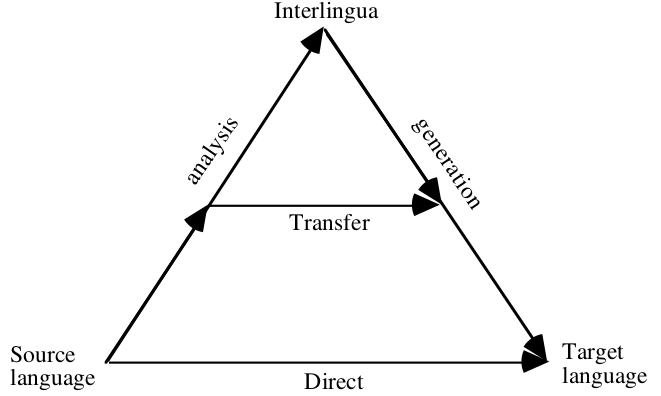
\includegraphics[scale=0.45]{images/interlingua.png}
\caption{Diagram outlining the three different Machine Translation strategies (Source: \cite{nicholas1996lojban})}
\end{figure}

Thankfully, one of the supporting articles about this claim gives us a very clear definition in its introduction:\newline

"(...) the source text is rendered in an abstract interlingua, a representational system able to do underlie both the source and the target
language, and from which the target language text could be directly generated."\footcite{nicholas1996lojban} \newline

This strategy has many theoretical advantages, the main one being that the number of required modules for machine translation are reduced when
applying this strategy. However, two concrete disadvantages stop this strategy from being used more often: defining a consistent interlingua is
extremely complicated, and disambiguation of the source text is often just as complex.\newline

In \citetitle{nicholas1996lojban}\footcite{nicholas1996lojban}, \citeauthor{nicholas1996lojban} posits that the ideal interlingua for Machine Translation would ressemble
greatly to Lojban in its approach to a rigid grammar which still includes labels to indicate abstract concepts such as attitudes or moods, but
indicates that Lojban is too "amateurish" and considers that it has too many flaws from a linguistics standpoint to be the solution.
He does, however, insist that designers of interlinguas for machine translation should really draw inspiration from Lojban.\newline 

Drawing from \citeauthor{nicholas1996lojban}, \citeauthor{immes2019lojbanic} takes an inspired approach in
\citetitle{immes2019lojbanic}\footcite{immes2019lojbanic}, where he creates "extensions" to Lojban called "Lojbanic English/Spanish/German".
With these, he creates a machine translation system through interlinguas, and concludes by presenting significant time reductions in translations
as opposed to regular methods of machine translation.\newline

For a very good article about this subject, but which unfortunately does not discuss Lojban, I advise the reader to explore
\citetitle{machinetranslationconlangs}\footcite{machinetranslationconlangs}. \newline

Another rather interesting article about using Lojban in the context of NLP is \citetitle{hintz2014semantic}\footcite{hintz2014semantic}. In it,
\citeauthor{hintz2014semantic} creates a very effective semantic parser in English, while using Lojban as a system to annotate the source text.

\newpage

\section{About Lojban as a tool for interaction between Humans, Computers and AIs}

Another usual claim to fame of Lojban is the theory that it could be a good language to improve Human-Computer interaction.\newline

An interesting approach to "Meet the computer halfway"\footcite{speer2004meeting} was suggested by researchers at the MIT. They postulate that it is easier
for a computer to "translate Lojban into a semantic representation than it is to do so with a natural language", and that it is easier
for a user to "learn a new human language than it is to learn a system's programming language", so both of them should communicate in Lojban.\newline

In the same vein, \citeauthor{goertzel2013lojban} suggests in \citetitle{goertzel2013lojban}\footcite{goertzel2013lojban} that a variation of Lojban,
which he names Lojban++, could be a suitable language for communication between humans and early-stage AGI (Artificial general intelligence)
systems.\newline

The same author goes even further and suggests, in \citetitle{goertzel2014communication}\footcite{goertzel2014communication}, that Lojban could be
an effective tool for AGIs to communicate between eachother.